\documentclass{beamer}                  %printtaukseen [handout]
\usetheme{Frankfurt}
\usecolortheme{dove}

%\usepackage{pgfpages}                          %printtaukseen
%\pgfpagesuselayout{2 on 1}[a4paper,border shrink=5mm]  %printtaukseen

\usepackage[T1]{fontenc}
\usepackage[utf8]{inputenc}
\usepackage{lmodern}


%highlighting
\usepackage{color}
\newcommand{\hilight}[1]{\colorbox{yellow}{#1}}

\usepackage{mathtools}
\usepackage{xfrac}
\usepackage[finnish, british]{babel}
\usepackage{cleveref}                       %for multiple refs in one ref
%\usepackage{luximono}
\renewcommand*\familydefault{\ttdefault} %% Only if the base font of the document is to be typewriter style
\usepackage{courier}




\usepackage[style=authoryear]{biblatex} %for citations
\bibliography{/Users/omojumiller/Dropbox/Research/Dissertation/dissertation}

\DeclareMathOperator*{\E}{\mathbb{E}}               % Expectation symbol


%%%%% PATHS %%%%%

\graphicspath{{figures/}}
\usepackage{subfig} % For subfigures in floats
%\addbibresource{refs.bib} %for citations

%%%% CUSTOMIZATION OF THE TEMPLATE %%%%%

\useinnertheme{rectangles} %rectangle bullets etc
\beamertemplatenavigationsymbolsempty   %no navigation bar
\setbeamercovered{transparent}      %future bullet points transparent 
\setbeamertemplate{frametitle}[default][colsep=-4bp,rounded=false,shadow=false] %no shadows
\definecolor{dark-gray}{gray}{0.80} %color for the navigation squares

%%%% FOOTLINE CUSTOMIZATION %%%%%

\setbeamercolor{section in head/foot}{fg=black, bg=white}
\makeatletter
\setbeamertemplate{footline}
{
  \leavevmode%
  \hbox{%
  \begin{beamercolorbox}[wd=.333333\paperwidth,ht=2.25ex,dp=1ex,center]{section in head/foot}%
    \usebeamerfont{author in head/foot}\insertshortauthor~~\beamer@ifempty{\insertshortinstitute}{}{(\insertshortinstitute)}
  \end{beamercolorbox}%
  \begin{beamercolorbox}[wd=.333333\paperwidth,ht=2.25ex,dp=1ex,center]{section in head/foot}%
    \usebeamerfont{title in head/foot}\insertshorttitle
  \end{beamercolorbox}%
  \begin{beamercolorbox}[wd=.333333\paperwidth,ht=2.25ex,dp=1ex,right]{section in head/foot}%
    \usebeamerfont{date in head/foot}\insertshortdate{}\hspace*{2em}
    \insertframenumber{} / \inserttotalframenumber\hspace*{2ex} 
  \end{beamercolorbox}}%
  \vskip0pt%
}

%%%% HEADER CUSTOMIZATION %%%%%


\setbeamertemplate{mini frame}
{%
  \begin{pgfpicture}{0pt}{0pt}{.1cm}{.1cm}
    \pgfpathrectangle{\pgfpointorigin}{\pgfpoint{\the\beamer@boxsize}{\the\beamer@boxsize}}
    \pgfusepath{fill,stroke}
  \end{pgfpicture}%
}

\def\slideentry#1#2#3#4#5#6{%
  %section number, subsection number, slide number, first/last frame, page number, part number
  \ifnum#6=\c@part\ifnum#2>0\ifnum#3>0%
    \ifbeamer@compress%
      \advance\beamer@xpos by1\relax%
    \else%
      \beamer@xpos=#3\relax%
      \beamer@ypos=#2\relax%
    \fi%
  \hbox to 2pt{%
    \beamer@tempdim=-\beamer@vboxoffset%
    \advance\beamer@tempdim by-\beamer@boxsize%
    \multiply\beamer@tempdim by\beamer@ypos%
    \advance\beamer@tempdim by -.05cm%
    \raise\beamer@tempdim\hbox{%
      \beamer@tempdim=\beamer@boxsize%
      \multiply\beamer@tempdim by\beamer@xpos%
      \advance\beamer@tempdim by -\beamer@boxsize%
      \advance\beamer@tempdim by 1pt%
      \kern\beamer@tempdim
      \global\beamer@section@min@dim\beamer@tempdim
      \hbox{\beamer@link(#4){%
          \usebeamerfont{mini frame}%
          \ifnum\c@section>#1%
            \color{dark-gray}%
          \else%
            \ifnum\c@section=#1%
              \ifnum\c@subsection>#2%
                \color{dark-gray}%
              \else%
                \ifnum\c@subsection=#2%
                  \ifnum\c@subsectionslide>#3%
                    \color{dark-gray}%
                  \else%
                    \color{fg}%
                  \fi%
                \else%
                  \color{dark-gray}%
                \fi%
              \fi%
            \else%
              \color{dark-gray}%
            \fi%
          \fi%
          \usebeamertemplate{mini frame}%
        }}}\hskip-10cm plus 1fil%
  }\fi\fi%
  \else%
  \fakeslideentry{#1}{#2}{#3}{#4}{#5}{#6}%
  \fi\ignorespaces
  }
  
%%%% SOME BUG %%%%%

\def\pdftex@driver{pdftex.def}
\ifx\Gin@driver\pdftex@driver
  \def\pgfsys@color@unstacked#1{%
    \pdfliteral{\csname\string\color@#1\endcsname}%
  }
\fi

\makeatother



%%%%% INFORMATION ABOUT THE DOCUMENT %%%%%

\title[Culturally Responsive CS]{Gaining Insights Into The Effects Of Culturally Responsive Curriculum On Historically Underrepresented Students’ Desire For Computer Science}
\author[Miller]{Omoju Miller}
\institute[UC Berkeley]{University of California, Berkeley }         
                      \date{June 2016}

                      
%%%%% ACTUAL DOCUMENT PAGES %%%%%                     

\begin{document}

\section{}
        \begin{frame}[plain]
            \titlepage 
        \end{frame}

\section{Challenge}
  \begin{frame}{}
    \begin{center}
      {\LARGE Equalizing Participation in Computer Science}
      \begin{enumerate}
                \item A lack of presence of CS in K-12 education.
                \item \textcolor{red}{\textbf{The \hilight{under-production} of post-secondary degrees in CS}}. 
                \item \textcolor{red}{\textbf{The underrepresentation of \hilight{women} in CS}}.
                \item The underrepresentation of ethnic minorities in CS.
                \item A lack of positive CS role models in the media. 
                
      \end{enumerate}
    \end{center}
  \end{frame}

\section{Design of an inclusive CS0 course at UC Berkeley}
        \begin{frame}{}
        Three pathways into CS at UC Berkeley
            \begin{itemize}
                \item \textcolor{red}{\textbf{CS3:\hilight{Introduction to Symbolic Programming}}}.
                \item CS61A: Structure and Interpretation of Computer Programs.
                \item CS61AS: Self paced version of CS61A
            \end{itemize}
        \end{frame}

        \begin{frame}{}
        In her study of attrition in undergraduate CS at Berkeley, Lewis found that female students were disproportionately weeded out of the track, often starting at CS3 \cite{Lewis:EECS-2010-132}.
        \end{frame}

        \begin{frame}{}
        Three pathways into CS at UC Berkeley
            \begin{itemize}
                 \item \textcolor{red}{\textbf{CS10:\hilight{The Beauty and Joy of Computing}}}.
                 \item CS61A: Structure and Interpretation of Computer Programs.
                \item CS61AS: Self paced version of CS61A
            \end{itemize}
        \end{frame}


\section{Research Methods}
\begin{frame}{}

  \begin{figure}[!htbp]
      \centering
      \subfloat[]{%
      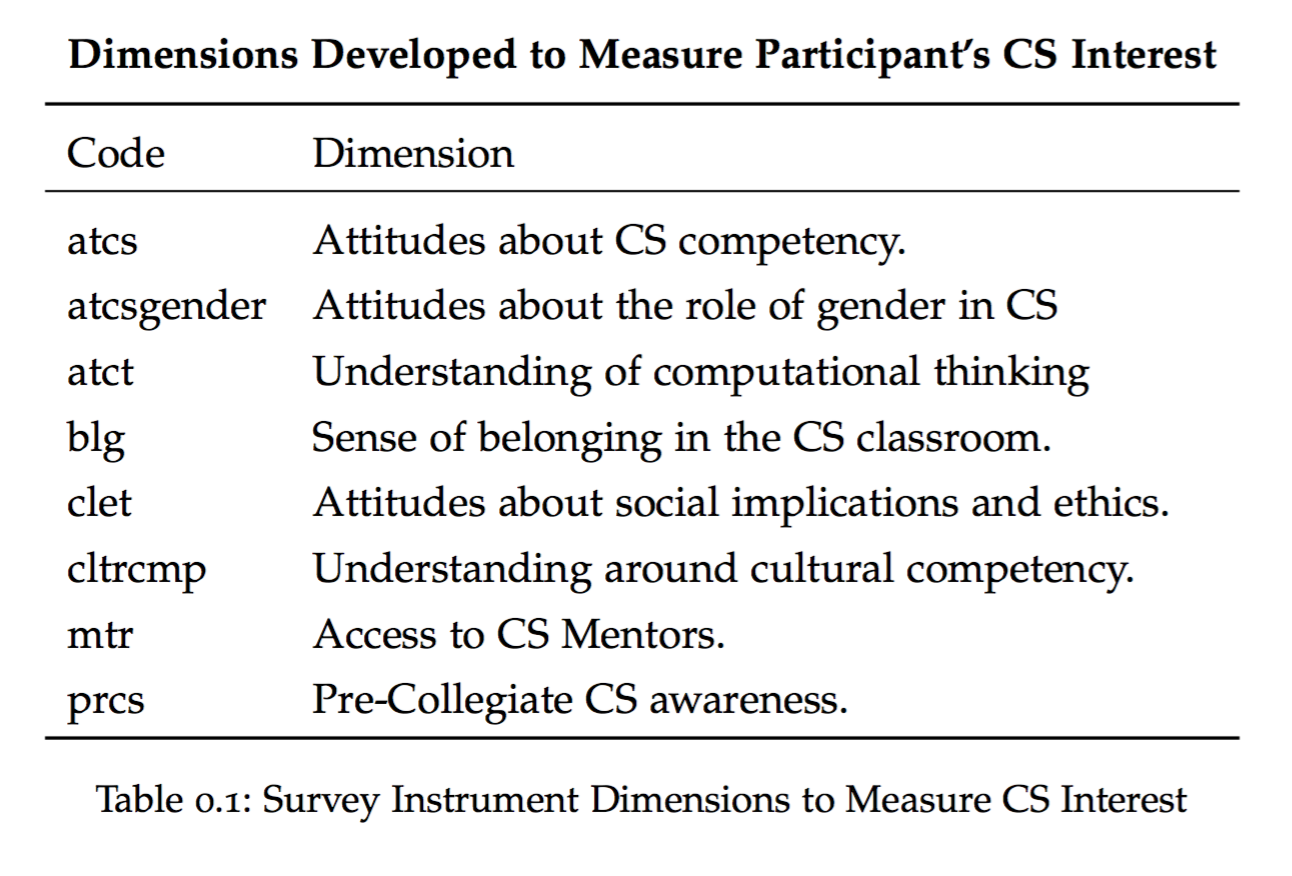
\includegraphics[width=1\textwidth]{CSAttitudes}
      }
      
  \end{figure}

\end{frame}

\section{Results}
\begin{frame}{Belonging}

\end{frame}

    

        
%----------------------------------------------------------------------------------------
%  REFERENCE LIST
%----------------------------------------------------------------------------------------

\printbibliography

\clearpage
\end{document}
              